%===========================================================
%                              Choix de thématique
%===========================================================
% Une des quatre options 'parallelisme', 'architecture', 'systeme' 
% 'tempsreel' doit être utilisée avec le style compas2021
\documentclass[parallelisme]{compas2022}
\usepackage{algorithm2e}

%===========================================================
%                               Title
%===========================================================

\toappear{1} % Conserver cette ligne pour la version finale

\begin{document}

\title{TCC}
\shorttitle{TCC}

\author{Saalik Hatia}%

\address{Université Pierre et Marie Curie\\
Laboratoire LIP6 \\
4, place jussieu\\
75005 Paris - France\\
saalik.hatia@lip6.fr}

\date{\today}

\maketitle

%===========================================================         %
%R\'esum\'e
%===========================================================  
\begin{abstract}
  Le fichier fonctionne en \LaTeXe. La taille
  de ce résumé peut atteindre une dizaine de lignes.
  \MotsCles{un maximum de 5 mots significatifs, en français, doivent être 
    isolés sous forme de mots-clés.}
\end{abstract}


%=========================================================
\section{Introduction}
%=========================================================

Modern planet-scale applications increasingly use database to provide users with fast, available and consistent data.
Developpers use these databases with complex backends to build fast and reliable applications.
Ideally we want databases to have fast writes and fast reads.
Fast writes are achieved using a journal; where newly written data is appended in a write only sequential log.
And fast read are achieved using a cache, where recently used version are stored in fast random access memory.

It is hard to achieve both, keeping everything in memory, or at least using memory as a first layer might cause data loss if there is a crash.
Similarly a journal is ideal if we think about data persistency, but reading through a sequential log can lead to high read latency.

Most databases, are build with these ideas in mind and have three major components that interact with each other:
\begin{itemize}
  \item Cache
  \item Version store
  \item Journal
\end{itemize}

On top of this if the database is geo distributed, there might be a replication layer that adds a new level of complexity on top the existing mecanisms.

% This paper present our work of formilising the behavior and  interaction between different component of a typical database.
% We start from an intuitive version of a database, an in memory key-value store that store object versions.
% We formalize the application programming interface (API) of that components and the effects each API has on the overall system.
% From these we add new components aiming to achieve feature parity to a real world database.

We adopt a stepwise approach.
The initial step studies a simplistic concurrent database system; we describe its key invariants, formalize an operational semantics, and provide a reference implementation.
Each following step adds a single feature.
We formalize the feature and show experimentally that the improved system simulates the simpler one.
This allows our final design to provide users with consistency guarantees while having an efficient backend in case of a recovery.
We claim to provide developers with a clear model that allows them to implement a correct and available database with features suited to their requirements.



% They expect their data to be consistency while remaining available.
% If a network partition or a crash were to occur they except being able to continue their work while disconnect and data to be safely merged and recovered.
% <!-- The majority of database use transactions to provide developpers with a simple and reliable way to interact with their data. -->
% Journaling, materializing, checkpointing, truncation and recovery are well-known mechanisms that can be used to maintain speed and consistency.
% Their interplay is known to be tricky and their implementation if often obscur.
% This leads to situation where a developper doesn't know what to expect just based on the different mechanisms used to implement t
% We wrote a formal model, came up with some simple design and we show through comparaison that this is true.

% Developpers use complicated backend to build their applications. 

%=========================================================
\section{Transaction and snapshots}
%=========================================================


Transactions are used in most modern database as a mean to execute multiple reads and writes operation.
Transactions are a set operation, reads and writes, that are terminated by an abort or a commit.
Operations are either reads which are read from a snapshot called \emph{Dependency Snapshot} defined at that start of the transaction or writes that have an effect on said snapshot. Add determinism to the transaction.
Visibility of these operations are defined by the consistency model used in the database.


\subsection{Transaction representation}

A transaction is represented using the following information:
\begin{itemize}
\item $\tau_i$ Unique transaction identifier.
\item $Dt$ Dependency timestamp which represent a snapshot the transaction will interact with.
\item $\varepsilon$ Effect map contains the writes made by the transactions.
\item $R$ Read set which records the keys of objects read by the transaction.
\item $Ct$ a commit timestamp that represent the time at which the timestamp has been committed.
\item $State$ a value that is either $live$ or $terminated$ representing the state of the transaction.\\
\end{itemize}

There are three main phases in the lifecycle of a transacton.
A transaction starts with a begin phase where the transaction is initialized, second the operational phase where the client execute operations and finally termination that ends the transaction.
During these phases a transaction goes through two state, \emph{live} and \emph{terminated}.

During the begin phase a transaction is assigned a unique identifier $\tau_i$ and a \emph{Dependency Snapshot Timestamp} ($dt$), while the Effect Map, Read Set and the commit timestamp are initialize at bottom ($\bot$).
At the end of the begin phase a transaction's state is set to \emph{live}.

During the operational phrase any number of arbitrary operations are executed.
Every Read triggers an update of the Read Set $R_i$ and every write triggers an update of the Effect Map $\varepsilon_i$.

Once all the operations are executed the transaction enters the termination phase where it either commits or abort depending on the client or the system invariants. 
At the end of this phase the transaction's state is set to \emph{terminated}

\subsection{Snapshot}

Snapshots are a collection of transactions that are represented by a timestamp $St$.
Each snapshot is composed of the transactions that have a commit timestamp $Ct \leq St$. 

Snapshots provide \emph{isolation} guarantees to the system, meaning a Client only reads object versions that are part of the snapshot and are committed. 
In addition to isolation, Snapshots also provide the client with \emph{atomicity} guarantees.
Meaning the effects of $\varepsilon_i$ of a transaction $\tau_i$ are seen in an all-or-nothing manner.

\subsection{Object-version}

The system maintains the following information about an object's version called Object-version: 
\begin{itemize}
  \item \emph{key} is the unique identifier of the object
  \item \emph{$\tau_i$} identifier of the transaction this version is materilized from
  \item \emph{blob} is a pointer to the value of the object materialized with the updates contained in the dependency snapshot of the transaction and its effect map
\end{itemize}

In this paper we will identify an Object-version in this manner $key_{\tau_i}$. \emph{(Bad wording)}

\section{Model}

% In order to model a the database we first define the main actors and interaction at play in a simple database.
% A database is a collection of data and accessed by a client.

We define two main actors in our system:
\begin{itemize}
  \item Client: Actor that interacts with a database using Application Programming Interfaces (APIs) exposed by the database
  \item Database: Actor that host data that is read and written by the client.
\end{itemize}


In this paper we will consider that connection to the database, and key discovery is out of scope.
Therefore a Client will only interact with the database through transactions.
To start and execute a transaction the Database exposes the following API:
\begin{itemize}
\item \emph{begin()} initialize a transaction with a snapshot (\emph{Dt})
\item \emph{read(key): blob} returns the object \emph{key} from the snapshot \emph{Dt}
\item \emph{effect(key,blob)} assigns a the value \emph{blob} to the key \emph{key}
\item \emph{abort()} abort the live transaction
\item \emph{commit()} assign a commit timestamp to the transaction and ends the transaction.
\end{itemize}

Starting from a simple in memory Key-Value store, we describe the model then progressively add features and compare every progression between them (\emph{figure \ref{fig:transitions}}).
We provide an implementation for every model and compare implementations between them to show that the implementation are equivalent.

\begin{figure}[tp]
  \centering
  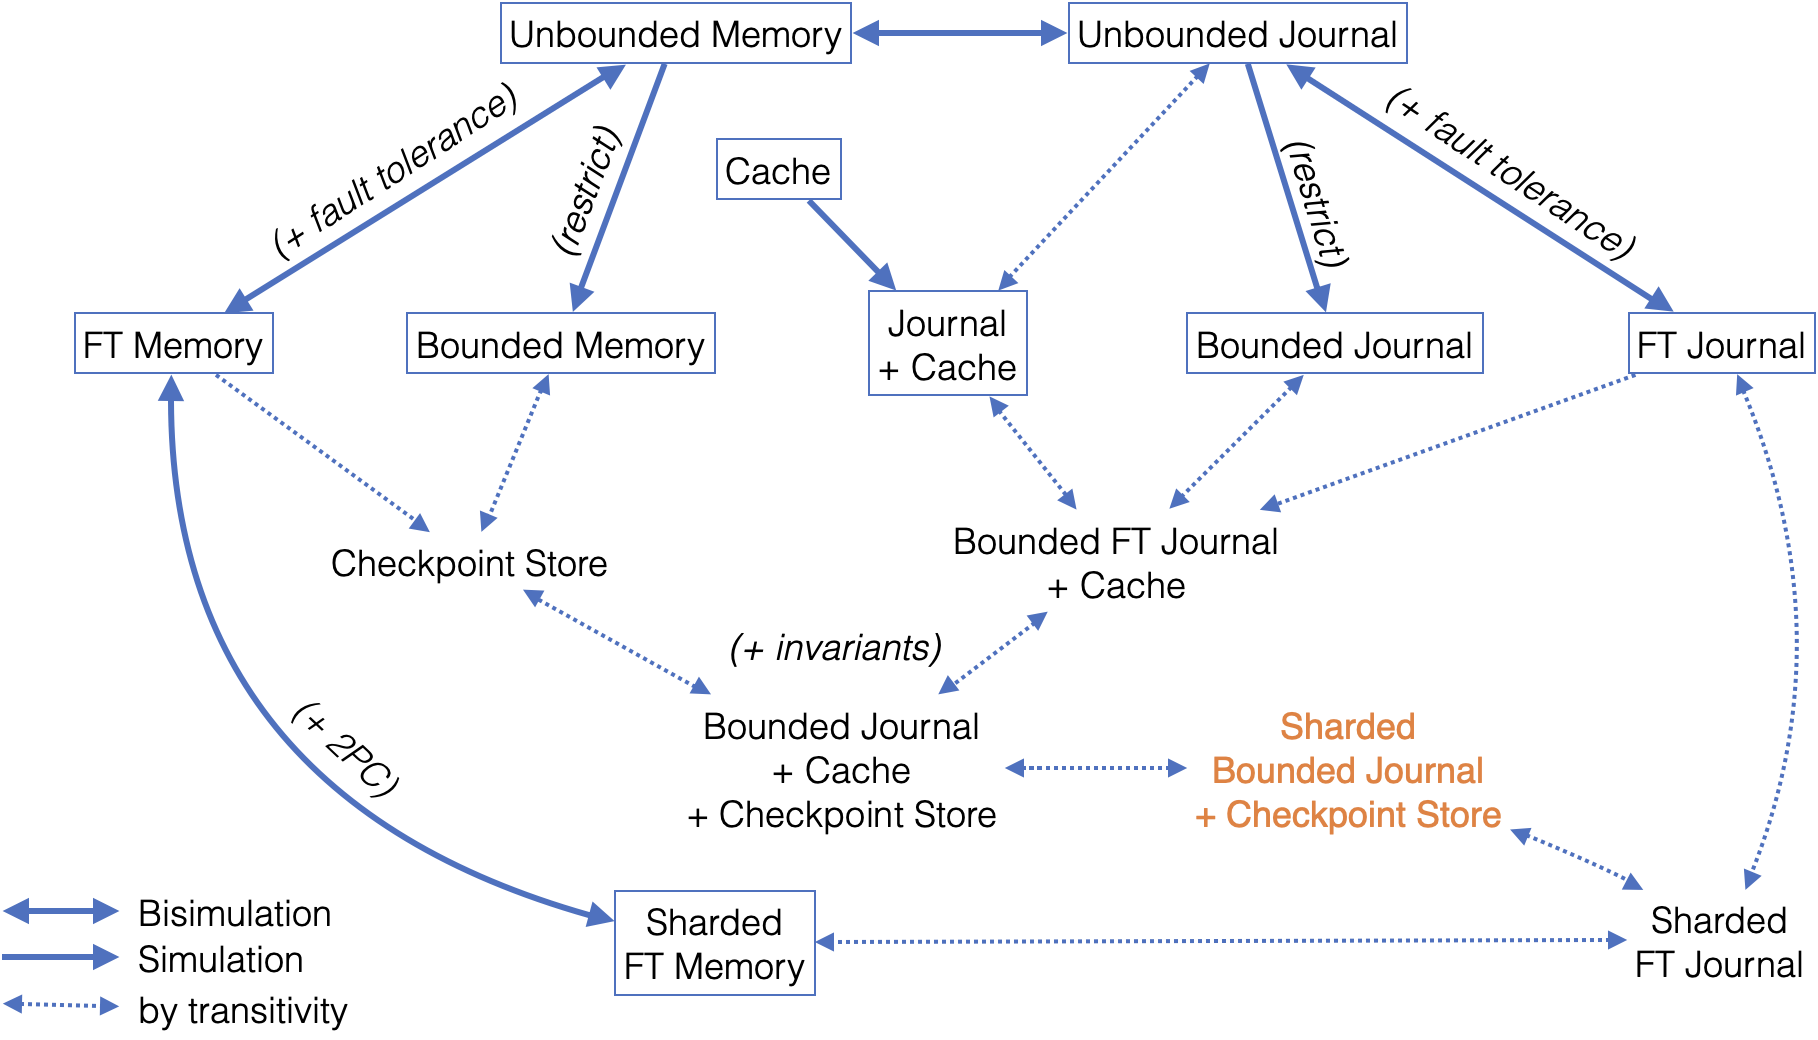
\includegraphics[width=0.75\textwidth]{figures/transitions.png}
  \caption{Progressions in our model}
  \label{fig:transitions}
\end{figure}

\subsection{Transactional Causal Consistency (TCC)}

Our model can be provide multiple conssitency level but in this work we focus our effort on TCC for every model.
To keep track of happened-before, we use timestamp to order updates.
Our model only having one data center, it is logically sequential.
When a transaction $\tau_i$ commits, it is assigned a timestamp that is the $Ct_i$.
This timestamp represent the point of visibility for all the effects $\varepsilon_i$ of the transaction.
If a transaction $\tau_j$ has a dependency $Dt_j$ higher than $Ct_i$ than all the effects of $\tau_i$ are visible for $\tau_j$.

Conflits are taken care of by using CRDTs as our data type ensuring that reading from a snapshot $St$ is determistic.

This model introduces our first system invariant which is that the commit timestamp of a transaction is always higher than the dependency timestamp.

\[
  \begin{array}{lcl}
    \emph{$Dt_i < Ct_i$}
  \end{array} 
\]

\subsection{Unbounded Memory}

The Unbounded Memory model stores Object-version $key_{\tau_id}$ in memory.
In adition to the object version the transaction information are also stored in memory in order to track information necessary to uphold our consistency guarantees.

Because this model is memory only, all data is lost is a crash or a restart happens.
Therefore there are no invariants regarding persistency or recovery.
Additionally we consider the memory to be unbounded so there are no restriction on the size of the data or constraints on the dependency timestamps.

\subsection{Transaction invariants}

For every transaction we define the following invariants.
In order to ensure that every operation is done within a transaction our model require that each API call except \emph{begin()} checks if there is a $live$ transaction for the calling client.

When a transaction commit it is causally dependent on the Snapshot reprensented by $Dt$.
We represent this by assigning a commit timestamp $Ct_i$ higher than the dependency timestamp.

These are the transaction invariants maintained during transactions:
\[
  \begin{array}{lcl}
    \emph{$Dt_i < Ct_i$}\\
    \emph{$(read, effect, commit, abort) => State = live$}
  \end{array} 
\]


TODO Le premier invariant est un peu faible tout seul. Il faut ajouter le fait qu'il est valable pour toutes transactions committées. Les sections suivantes sont sous forme de texte mais elle seront mise sous forme de pseudo code avec les precondition et les invariants.\\


\textbf{Start transaction}
When a client starts a transaction, if the client specify a dependency timestamp $Dt$ the system checks if it is valid in regards to consistency guarantees and creates a transaction object.
If no dependency timestamp is specified than the transaction is initialized with a valid dependency timestamp.
The transaction is then assigned a unique transaction identifier $\tau_i$ and $\emph{State} \leftarrow \emph{live}$ \\

Postconditions:\\
$State_i \leftarrow \emph{live}$ \\


\textbf{Read}\\
Preconditions:\\ 
$State_i = \emph{live}$ \\

Returns the Object-version k from the snapshot \emph{Dt}. 
If the object doesn't exist the system returns a default value.

In case a transaction attempts to read an object that has concurrent updates, we use CRDTs in order to ensure that the merge is determistic.
The system adds the key to the read set of the live transaction.\\
$R_i \leftarrow \emph{key}$\\

\textbf{Effect}\\
Preconditions:\\ 
$State_i = \emph{live}$ \\

Applies the effect on the object present in the snapshot \emph{dt} resulting in the creation of a new object-version.
The object version is then added to the Effect Map of the live transaction.\\
$\varepsilon \leftarrow key_{\tau}$

\textbf{Commit transaction}\\
Preconditions:\\ 
$State_i = \emph{live}$ \\

When a transaction is committed the system checks if the transaction is valid in regard to the consistency model chosen by the system.
If everything is correct then the transaction is committed and the transaction is assigned a commit timestamp such as $Dt_i \leq Ct_i$.

All the effects of the transaction are then available for transaction that have $Dt_j \geq Ct_i$.\\

Postconditions:\\
$State_i \leftarrow \emph{terminated}$ \\
$Dt_i \geq Ct_i$.\\



\textbf{Abort transaction}
Preconditions:\\ 
$\emph{State} = \emph{live}$ \\

If a transaction is aborted then all the effects of the transaction are void.

Postconditions:\\
$State_i \leftarrow \emph{terminated}$ \\

\subsection{Bounded Memory}

In the Bounded Memory model we choose to define an arbitrary limitation on the size of the memory used by the system.

\textbf{System invariants}
All system invariants from the Unbounded memory are present here.
Plus we introduce a two new value:
\begin{itemize}
  \item \emph{$M_{used}$} contains the current size of data in memory
  \item \emph{$M_{limit}$} represents the maximum size available to the database
\end{itemize}
Based on these two variable we introduce a new system invariant:
\begin{itemize}
  \item \emph{$M_{used}$} $<$ \emph{$M_{limit}$}
\end{itemize}
In order to uphold the memory constraints of the system we keep track of all the dependencies of running transactions called \emph{RunningTr} but also all the commit timestamps of finished transactions \emph{CommitTr}.

We then introduce a new timestamp called Minimum Dependency \emph{MinDt}.
\emph{MinDt} represents the oldest snapshot any running transaction is reading from.
When a transaction $\tau_i$ commits or aborts, it is removed from \emph{RunningTr}. 
And if $Dt_i = MinDt$ and no other transaction is reading from $Dt_i$ the system advances \emph{MinDt} to the next oldest snapshot used in \emph{RunningTr}.


\subsection{Garbage collection}
When \emph{$M_{used}$} $\geq$ \emph{$M_{limit}$}. 
All the transaction in the system are halted in order to perform a garbage collection.

Ici je dois expliquer comment est fait le GC:\\
\begin{algorithm}
  \KwIn{\\ \Indp
  RunningTr : set
  }
  \(oldTr \longleftarrow \emptyset\)\;
  % \ForAll{$\tau_i$ $\in$ Running}{
  %   \If{$Dt_i < MinDt$}{
  %     \(oldTr \longleftarrow $\tau_i$\)\;
  %   }
  % }
\end{algorithm}

% oldTr <- \{\}\\
% For each $\tau_i$ $\in$ Running:\\
%   if $Dt_i < MinDt$:\\

  % \begin{algorithm}
  %   \caption{Selection of relays, static MPR}
  %   \KwIn{\\ \Indp
  %     \(N_{1}\) : \textit{set}\\
  %     \(N_{2}[]\) : \textit{map} (\(n_{i} \in\ N_{1}\)) \(\rightarrow \{n_{k},...\}\)
  %   }
  %   \(U \longleftarrow \bigcup\limits_{n_{i} \in N_{1}}\) \(N_{2}[n_{i}]\)\;
  %   \(R \longleftarrow \emptyset\)\;
  %   \ForAll{\(n_{i} \in N_{1}\)}{
  %     \If{\(\exists n_{\text{iso}} \in N_{2}[n_{j}] \mid \forall n_{k \ne j}, n_{\text{iso}} \notin N_{2}[n_{k}]\)}{
  %        \(R \longleftarrow R \cup \{n_{j}\}\)\;
  %        \(U \longleftarrow U \setminus N_{2}[n_{j}]\)\;
  %     }
  %   }
  %   \While{\(U \ne \emptyset\)}{
  %     select \(n_{j} \in N_{1}\) maximizing \(\vert H_{2}[n_{j}] \cap U \vert\)\;
  %     \(R \longleftarrow R \cup \{n_{j}\}\)\;
  %     \(U \longleftarrow U \setminus N_{2}[n_{j}]\)\;
  %   }
  %   \Return{\(R\)}\;
  % \end{algorithm}


\subsection{Implementation}

Every model is implemented in java with external libraries for persistency, CRDTs and data structures that we consider being correct.
Implementation and evaluation of the different models have two purposes.
First we implement our different models as closely as possible to our specification and show that they are correct by running the same test on all versions.

Finally we plan on designing test that specifically targets breaking invariants defined in our model making sure the system crashes if they are violated, and run a set of traces that are generated from a Coq implementation.



\section{Conclusion}


\bibliography{exemple}

\end{document}